% !TEX encoding = UTF-8 Unicode
\documentclass{standalone}
% \usepackage{pgfplots}
% \pgfplotsset{compat=1.11}
\usepackage{amsmath}
\usepackage{amsfonts}
\renewcommand{\familydefault}{\sfdefault}
% \usepackage[version=0.96]{pgf}
\usepackage{tikz}
\usetikzlibrary{patterns}
% \usetikzlibrary{arrows,shapes,automata,backgrounds,petri,positioning}
% \usetikzlibrary{decorations.pathmorphing}
% \usetikzlibrary{decorations.shapes}
% \usetikzlibrary{decorations.text}
% \usetikzlibrary{decorations.fractals}
% \usetikzlibrary{decorations.footprints}
% \usetikzlibrary{shadows}
% \usetikzlibrary{calc}
% \usetikzlibrary{spy}

% \pgfplotsset{compat=1.11}
\usepackage[utf8]{inputenc}
% \usepackage[vietnam]{babel}

\def\d{.6}
% \def\p{5.1}
\def\q{-.6}
% \def\sc{25}

\newcommand{\nn}[4]{
    \begin{scope}[xshift = #1*\d cm, yshift = #2*\q cm]
        
    \node at (0, 0) [anchor = east, draw, inner sep = 0, fill = #3!20, minimum height = .6cm, minimum width = .6cm] {#4};
    \end{scope}
}

\newcommand{\nnn}[4]{
    \begin{scope}[xshift = #1*\d cm, yshift = #2*\q cm]
        
    \node at (0, 0) [anchor = east, align = left,  draw, inner sep = 0, fill = #3!30, minimum height = .6cm, minimum width = .6cm] {#4};
    \end{scope}
}

\tikzstyle{shaded0}=[pattern = north east lines, fill opacity = .2, thick]
\tikzstyle{shaded1}=[pattern = dots, fill opacity = .2, thick]
\tikzstyle{shaded2}=[pattern = grid, fill opacity = .2, thick]

\begin{document}
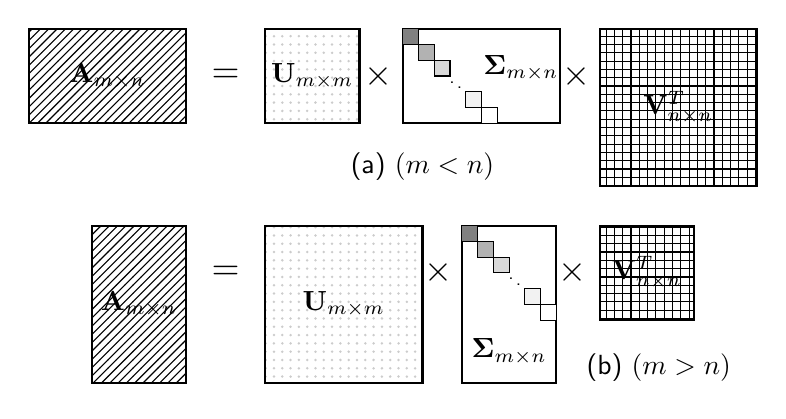
\begin{tikzpicture}
    \begin{scope}
        \def\m{1.2}
        \def\n{2}
        \def\d{.2}
        \begin{scope}
            \draw [shaded0] (0, 0) rectangle (\n, -\m);
            \node at (0.5*\n, -0.5*\m) {$\mathbf{A}_{m \times n}$};
            \node [scale = 1.3] at (1.25*\n, -0.5*\m) {=};
        \end{scope}

        \begin{scope}[xshift = 3 cm]
            \draw [shaded1] (0, 0) rectangle (\m, -\m);
            \node [scale = 1.3] at (1.2*\m, -0.5*\m) {$\times$};
            \node at (0.5*\m, -0.5*\m) {$\mathbf{U}_{m \times m}$};

        \end{scope}


        \begin{scope}[xshift = 4.75 cm]
            \draw [thick] (0, 0) rectangle (\n, -\m);
            \draw [fill = gray!100] (0*\d, 0*\d) rectangle (1*\d, -1*\d);
            \draw [fill = gray!60]  (1*\d, -1*\d) rectangle (2*\d, -2*\d);
            \draw [fill = gray!30]  (2*\d, -2*\d) rectangle (3*\d, -3*\d);
            \node [scale = .7] at (3.6*\d, -3.4*\d) {$\ddots$};
            \draw [fill = gray!10]  (4*\d, -4*\d) rectangle (5*\d, -5*\d);
            \draw [fill = gray!0]   (5*\d, -5*\d) rectangle (6*\d, -6*\d);
            \node at (0.75*\n, -.25*\n) {$\mathbf{\Sigma}_{m \times n}$};

            \node [scale = 1.3] at (1.1*\n, -0.5*\m) {$\times$};
        \end{scope}

        \begin{scope}[xshift = 7.25 cm]
            \draw [shaded2] (0, 0) rectangle (\n, -\n);
            \node at (0.5*\n, -0.5*\n) {$\mathbf{V}^T_{n \times n}$};
        \end{scope}
        \node at (5, -1.75) {(a) $ (m < n)$};
    \end{scope}

    \begin{scope} [yshift = -2.5cm]
        \node at (8, -1.8) {(b) $(m > n)$};
        \def\m{2}
        \def\n{1.2}
        \def\d{.2}
        \begin{scope}[xshift = .8cm]
            \draw [shaded0] (0, 0) rectangle (\n, -\m);
            \node at (0.5*\n, -0.5*\m) {$\mathbf{A}_{m \times n}$};
            \node [scale = 1.3] at (.85*\m, -0.5*\n) {=};
        \end{scope}

        \begin{scope}[xshift = 3 cm]
            \draw [shaded1] (0, 0) rectangle (\m, -\m);
            \node [scale = 1.3] at (1.1*\m, -0.5*\n) {$\times$};
            \node at (0.5*\m, -0.5*\m) {$\mathbf{U}_{m \times m}$};

        \end{scope}


        \begin{scope}[xshift = 5.5 cm]
            \draw [thick] (0, 0) rectangle (\n, -\m);
            \draw [fill = gray!100] (0*\d, 0*\d) rectangle (1*\d, -1*\d);
            \draw [fill = gray!60]  (1*\d, -1*\d) rectangle (2*\d, -2*\d);
            \draw [fill = gray!30]  (2*\d, -2*\d) rectangle (3*\d, -3*\d);
            \node [scale = .7] at (3.6*\d, -3.4*\d) {$\ddots$};
            \draw [fill = gray!10]  (4*\d, -4*\d) rectangle (5*\d, -5*\d);
            \draw [fill = gray!0]   (5*\d, -5*\d) rectangle (6*\d, -6*\d);
            \node at (.5*\n, -.8*\m) {$\mathbf{\Sigma}_{m \times n}$};

            \node [scale = 1.3] at (.7*\m, -0.5*\n) {$\times$};
        \end{scope}

        \begin{scope}[xshift = 7.25 cm]
            \draw [shaded2] (0, 0) rectangle (\n, -\n);
            \node at (0.5*\n, -0.5*\n) {$\mathbf{V}^T_{n \times n}$};
        \end{scope}
    \end{scope}
\end{tikzpicture}
\end{document}